\subsection{Analyse der bestehenden Strukturen und Prozesse}
\label{subsec:analyse-der-bestehenden-strukturen-und-prozesse}

In diesem Unterkapitel wird der Aufbau der automatisch
generierten Testberichte aus dem Teststand und der vorhandenen Ausgabe- und Speicherstruktur
erläutert. Dies ist relevant für die Erstellung der Datenbank und das
Verständnis der Ein- und Auslesefunktionen der Web-Applikation.

\subsubsection{XML-Berichtsstrukturschema}

Die vom Teststand automatisch generierten
Berichte folgen einem konstanten Strukturschema, welches sich bis zu einer
gewissen Ebene der XM-Struktur in jedem Bericht wiederholt. Wie im Kapitel „Grundlagen“
beschrieben, kann ein Element Attribute, andere Elemente und einen Inhaltswert beinhalten.

Das Stammelement heißt in allen automatisch
generierten Berichten „test“ und besitzt immer das Attribut „id“. Die Zahl in
diesem Attribut beschreibt die Art des \ac{DUTs}.

Das Stammelement hat die Unter- bzw.
Kinderelemente „info“, „testbench“, „string“ und dreimal „testmodule“. Diese
Elemente haben wiederum alle weiter Unterelemente und Attribute.

Jedes der Elemente „testmodule“ hat ein Attribut
„name“, durch welches Sie unterschieden werden können. Das Element „string“ hat
ein Namensattribut mit der Bezeichnung „test sequence status“. Der Inhalt
dieses Elementes gibt an, ob der Test erfolgreich abgeschlossen wurde oder ob
es einen Fehler bzw. eine Grenzüberschreitung von Messwerten gab.
Die hier genannten eigenschaften sind in der Abbildung \ref{fig:3. XML-Strukturbeispiel Kinder der Stammelementes} zu erkennen.

\begin{figure}[h]
    \centering
    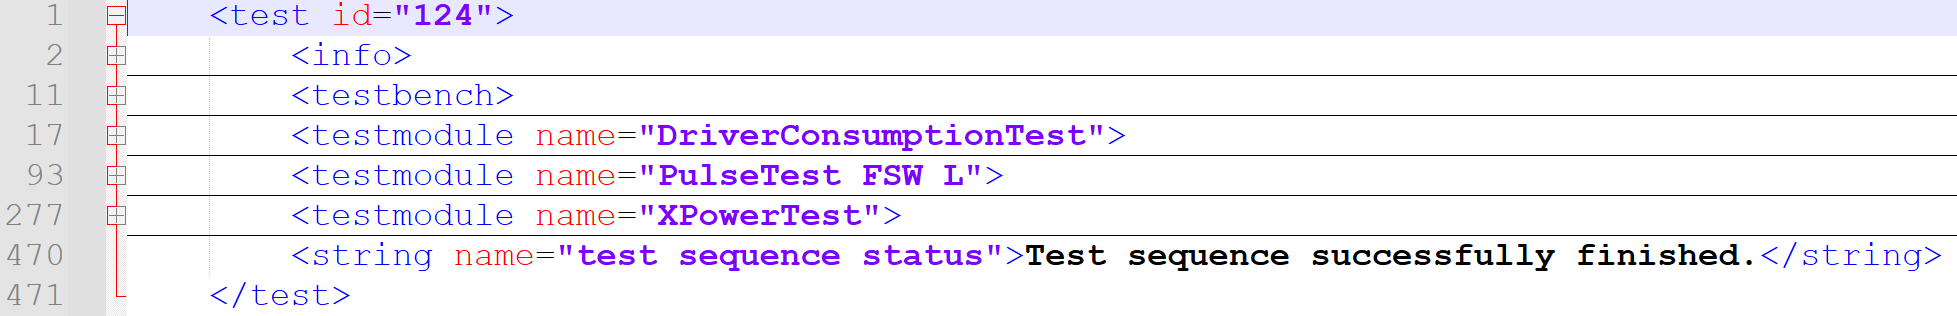
\includegraphics[width=0.8\textwidth]{Grafiken/Obere_XML-Berichtstruktur(1)}
    \caption{Aufbau des Teststandes}
    \label{fig:3. XML-Strukturbeispiel Kinder der Stammelementes}
    {Quelle: Eigene Aufnahme aus Nootpad++}
\end{figure}


